\section{Transformation Plan}
\label{sec:transformation_plan}
With the gaps defined in \fref{sec:gaps}, these can now be divided up and translated into key work packages essential for realising the envisioned architecture. Additionally, the work packages are then depicted in a gantt diagram; the purpose of this is twofold,  to estimate the duration of each work package as well as getting a sense for the internal dependencies among them.
%
\subsection{Activities}
In the following three tables the activities associated with respective model (claim, order and support) are listed. For each table the activities are ordered by execution priority, i.e. activities are executed top-down.
\begin{table}[H]
	\centering
	\begin{tabular}{|c|p{3cm}|p{10.5cm}|}
		\hline
		\textbf{\#} & \multicolumn{1}{c|}{\textbf{Role}} & \multicolumn{1}{c|}{\textbf{Activity}} \\ \hline
		\textbf{1} &  & Develop the new website functionality \\ \hline
		\textbf{2} &  & Integrate website with existing CRM DB\\ \hline
		\textbf{3} &  & Deploy beta version in parallel with existing system and review test run \\ \hline
		\textbf{4} &  & Deploy production version of the new functionality of the website \\ \hline
		\textbf{5} &  & Replace the order manager with the automated order registration process. And remove Order management system\\ \hline

	\end{tabular}	
	\caption{"Order" activities}
	\label{table:activities_order}
\end{table}

\begin{table}[H]
	\centering
	\begin{tabular}{|c|p{3cm}|p{10.5cm}|}
		\hline
		\textbf{\#} & \multicolumn{1}{c|}{\textbf{Role}} & \multicolumn{1}{c|}{\textbf{Activity}} \\ \hline
		\textbf{1} &  & Analyze how to proceed with the website functionality extension. Who, what and when are questions answered here  \\ \hline
		\textbf{2} &  & Proceed with development of "Customer Claim Portal" and integrate this with Claim Management system\\ \hline
		\textbf{3} &  & Review system and ensure function and service compatibility \\ \hline
		\textbf{4} &  & Deploy beta version to website and test run \\ \hline
		\textbf{5} &  & Release the new Claim portal of the website\\ \hline
		\textbf{6} &  & Remove claim administrator as well as functions and services related to form downloading\\ \hline
	\end{tabular}	
	\caption{"Claim" activities}
	\label{table:activities_claim}
\end{table}

\begin{table}[H]
	\centering
	\begin{tabular}{|c|p{3cm}|p{10.5cm}|}
		\hline
		\textbf{\#} & \multicolumn{1}{c|}{\textbf{Role}} & \multicolumn{1}{c|}{\textbf{Activity}} \\ \hline
		\textbf{1} &  & Analyze benefits and drawbacks of developing or buying combined Helpdesk system \\ \hline
		\textbf{2} &  & Procure combined helpdesk system\\ \hline
		\textbf{3} &  & Integrate helpdesk system, phone system dispatcher and mail server \\ \hline
		\textbf{4} &  & Ensure that functionality and service support are maintained \\ \hline
		\textbf{5} &  & Deploy support system in a test environment\\ \hline
		\textbf{6} &  & Educate staff how to use the new system\\ \hline
		\textbf{7} &  & Engage transition period by having both systems running in parallel\\ \hline
		\textbf{8} &  & Remove old Phone Support System \& DB and Mail Support System \& DB\\ \hline
	\end{tabular}	
	\caption{"Support" activities}
	\label{table:activities_support}
\end{table}


\subsection{Gantt Scheme}
\begin{center}
	\begin{figure}[H]
		\centering
		\setlength\fboxsep{7pt}
		\setlength\fboxrule{0.5pt}
		\fbox{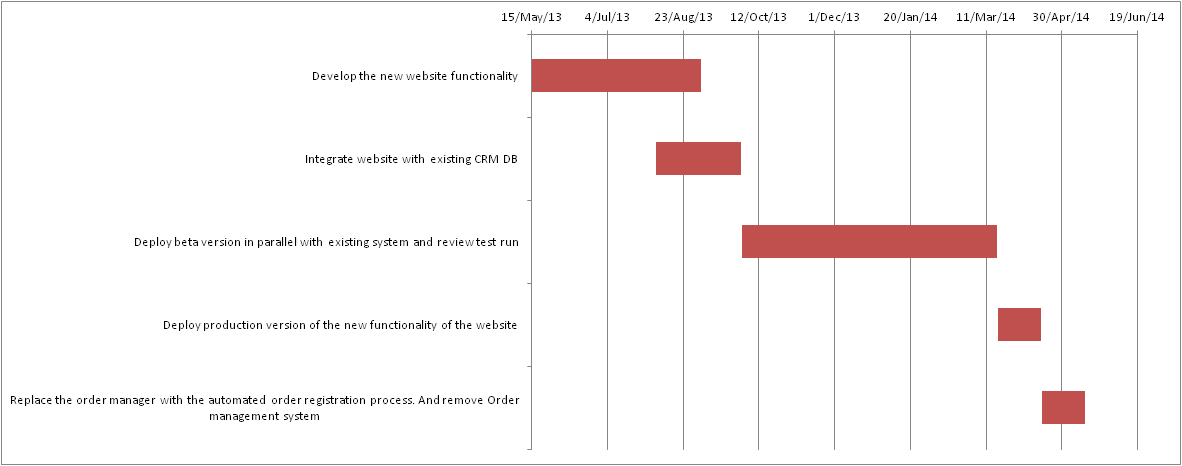
\includegraphics[scale = 0.5, angle=90]{images/gant_order.png}}
		\caption{Gantt chart for "Order" activities}
		\label{fig:gant_order}
	\end{figure}
\end{center}
\begin{center}
	\begin{figure}[H]
		\centering
		\setlength\fboxsep{7pt}
		\setlength\fboxrule{0.5pt}
		\fbox{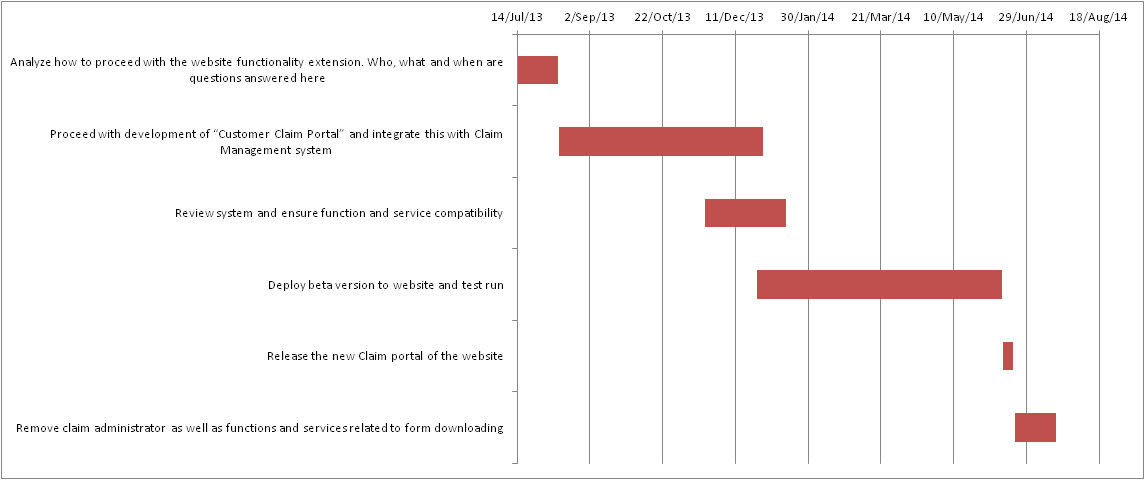
\includegraphics[scale = 0.5, angle=90]{images/gant_claim.png}}
		\caption{Gantt chart for "Claim" activities}
		\label{fig:gant_claim}
	\end{figure}
\end{center}

\begin{center}
	\begin{figure}[H]
		\centering
		\setlength\fboxsep{7pt}
		\setlength\fboxrule{0.5pt}
		\fbox{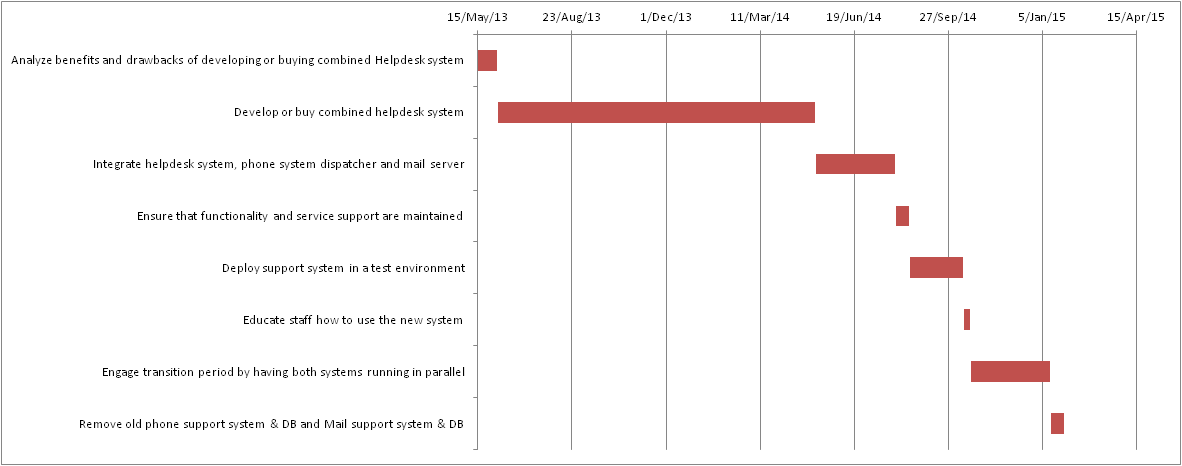
\includegraphics[scale = 0.5, angle=90]{images/gant_support.png}}
		\caption{Gantt chart for "Support" activities}
		\label{fig:gant_support}
	\end{figure}
\end{center}